%%%%%%%%%%%%%%%%%%%%%%%%%%%%%%%%%%%%%%%%%%%%%%%%%%%%%%%%%%%%%%%%%%%%%%%%%%%%%%%%
\section{Discussion}

%%%%%%%%%%%%%%%%%%%%%%%%%%%%%%%%%%%%%%%%%%%%%%%%%%%%%%%%%%%%%%%%%%%%%%%%%%%%%%%%
\subsection{Proposed TR WPT System}
\label{sec:WPTSys}

This research is part of an exploration of time reversal applied to WPT applications. Our proposed WPT system is shown in Fig.~\ref{fig:SysImage}. This research investigates one particular performance parameter of the system. However, many unknowns regarding the design and performance of the TR WPT system remain.

\begin{figure}[t!]
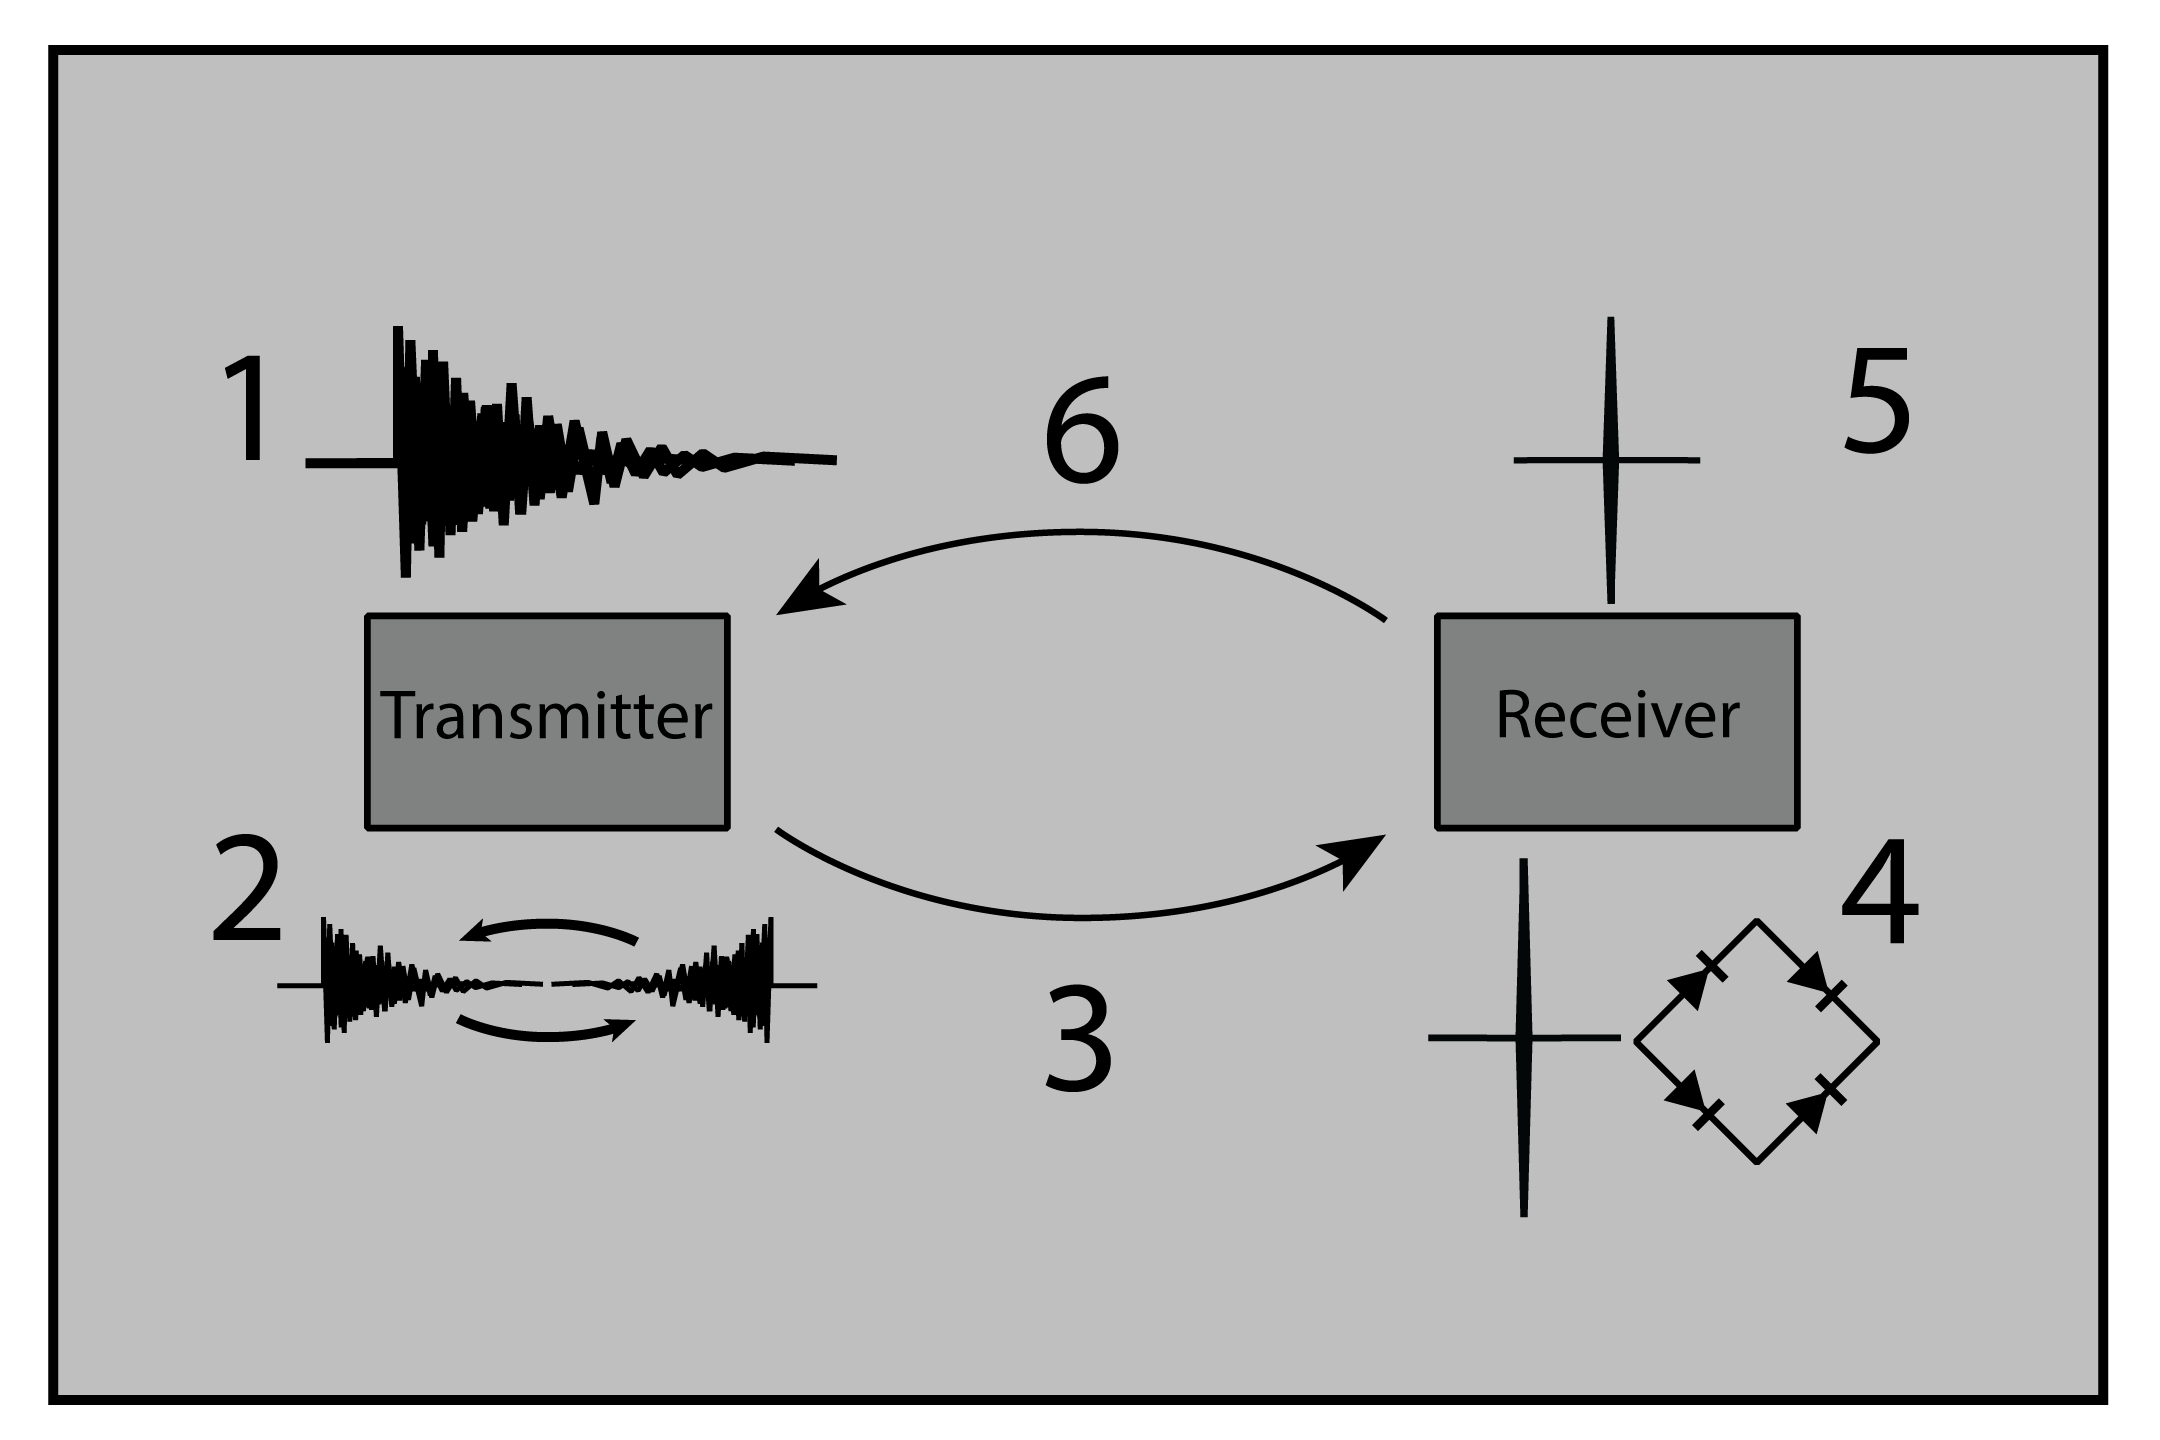
\includegraphics[width=\columnwidth]{figs/WPTSys.png}
\caption{The proposed time reversal system. The system begins by detecting a sona from a valid target (1). The sona is time-reversed (2) and broadcast back into the environment (3). The signal reconstructs on the receiver, which rectifies the energy (4).  A small amount of the energy is used to broadcast a new signal (5) into the environment (6) and the cycle repeats.}
\label{fig:SysImage}
\end{figure}

\todo{Bulleted List for the paragraphs below?}

The proposed TR WPT system has three basic components. The first is a rectenna that serves as the receiver of the WPT system. ~\cite{FRAZIER} and ~\cite{ROMAN} \todo{Fix citations. Are we allowed to cite Scott?} demonstrate how individual receivers in a group can be focused on.

The second system component is a transmitter that performs the time reversal process.  This system will detect the identify signals from the receiver(s), time reverse the signals, and broadcast them. \todo{Awkward wording}  How the processing speed of identification and time reversal affects system performance is the main focus of this research.

Time reversal is heavily dependent on environmental factors.  Thus, the environment should be considered a component in the design of a TR WPT system.  TR must occur in a scattering environment to work effectively.  A low-loss system is also necessary to maximize the transfer efficiency. We found that approximately X\% of energy \todo{GET THIS NUMBER} transmitted through our test cavity was lost due to environmental factors. Some environmental modifications will be need to be made during the installation of a TR WPT system.

\subsection{Contributions}
\label{sec:Contrib}
\todo{Is this too tacky a subsection?}

In the above experiments, we demonstrate the shape of the spatial profile of electromagnetic
TR. This profile takes the form \texttt{|sinc(x)|}, dependent on wavelength $b$.
Additionally, the ability of a TR system to transmit energy to a moving target is 
demonstrated to be dependent on this profile, and the transmission dead 
time of $t_{d}$.

Any WPT system utilizing time reversal will have to account for the 
finite-size bubble of fields around  the  main  reconstruction  point.
Methods  have  been developed  to  improve  the  spatial  focusing  of  reconstructions
well below the diffraction limit [11].

The team’s experimental TR system is not optimized for downtime; currently a
single TR operation takes approximately 7 seconds.  However, the researchers 
believe that this number can be significantly improved in a finalized TR WPT 
system, allowing for effective power transfer at speeds must faster than those 
considered here.

Additionally, we propose that understanding and characterizing how environmental 
factors impact TR is a major obstacle to the design of a TR WPT system. Environmental
effects should be a major research priority accordingly.
\
Based on the results shown in Fig.~\ref{fig:moving_recon}, we would further
expect the reconstruction amplitude to vary over a wider range as the velocity
of the target increases
%
Nevertheless we believe one of the main advantages of time reversal over
existing WPT methods is its ability to track moving
targets~\cite{fink,nltr-wave-chaotic}.
%%%%%%%%%%%%%%%%%%%%%%%%%%%%%%%%%%%%%%%%%%%%%%%%%%%%%%%%%%%%%%%%%%%%%%%%%%%%%%%%

%%%%%%%%%%%%%%%%%%%%%%%%%%%%%%%%%%%%%%%%%%%%%%%%%%%%%%%%%%%%%%%%%%%%%%%%%%%%%%%%
\subsection{Limitations and Future Work}
\label{sec:limitations}


These experiments were limited primarily by the environment and equipment used
for testing.
%
A consumer electronics environment is likely to be much larger than the chamber
used in this study, and filled with clutter.
%
Both of these properties would improve the modal density of the environment,
creating more transmission channels between source and target, ultimately
improving reconstruction quality.
%
On the other hand, such environments would likely have significantly larger loss
than those considered in our experiments.



%Our results show that time reversal mirrors may be able to effectively
%exploit multiple channels, but we leave this to future work.
%Great benefit can also be achieved by utilizing multi-channel time reversal mirrors.
%Understanding how
%to maximize the effectiveness of these technologies while minimizing cost is
%critical.



The single-channel time reversal method is limited in the amount of power it can
transmit to a target.
%
It is certainly sufficient to perform long-term trickle charging or to act as a
secondary-source of energy extending battery life.
%
A multi-channel realization of time reversal will be able to deliver much
greater time-integrated power.



The theoretical limit for the speed of the time reversal process needs to be
determined.
%
These experiments were severely limited by the processing time of the combined
MATLAB-DSO-AWG-PSG test and measurement system.
%
Dedicated hardware and firmware would eliminate communication overhead and thus
dramatically improve the speed of the WPT process presented here.
%%%%%%%%%%%%%%%%%%%%%%%%%%%%%%%%%%%%%%%%%%%%%%%%%%%%%%%%%%%%%%%%%%%%%%%%%%%%%%%%
